\documentclass[a4paper]{report}

%uncomment to see the references
%\usepackage{showkeys}
\usepackage[T2A]{fontenc}

\usepackage[section]{algorithm}
\usepackage{algorithmic}
\usepackage[english,russian]{babel}
\usepackage{framed}
\usepackage{nomencl}

\usepackage[backend=bibtex,bibencoding=utf8,sorting=none,sortcites=true,bibstyle=sty/gost71,maxnames=99,citestyle=numeric-comp,babel=other]{biblatex}

\defbibenvironment{bibliography}
  {\listoffigures
     {\printfield[labelnumberwidth]{labelnumber}.}
     {\setlength{\labelwidth}{2\labelnumberwidth}%
      \setlength{\leftmargin}{\labelwidth}%
      \setlength{\labelsep}{\biblabelsep}%
      \addtolength{\leftmargin}{\labelsep}%
      \setlength{\itemsep}{\bibitemsep}%
      \setlength{\parsep}{\bibparsep}}%
      \renewcommand*{\makelabel}[1]{\hss##1}}
  {\endlist}
  {\item}

\usepackage[utf8]{inputenc}
\usepackage{csquotes}
%\usepackage{expdlist}
%\usepackage[nottoc,notbib]{tocbibind}
\usepackage[pdftex]{graphicx}
\usepackage{graphicx}
\graphicspath{{pic/}}
\usepackage{amsmath}
\usepackage{amssymb}
\usepackage{amsthm}
\usepackage{amsfonts}
\usepackage{amsxtra}
\usepackage{sty/dbl12}
%\usepackage{srcltx}
\usepackage{epsfig}
% \usepackage{verbatim}
\usepackage{sty/rac}
\usepackage{listings}
\usepackage{sty/scala}
\usepackage[singlelinecheck=false]{caption}
\usepackage{multirow}

\usepackage{xcolor, colortbl}

\definecolor{light-gray}{RGB}{230,230,230}
\definecolor{dkgreen}{RGB}{0,154,0}
\definecolor{gray}{RGB}{128,128,128}
\definecolor{mauve}{RGB}{149,0,210}
\definecolor{purpur}{RGB}{255,204,153}
%%%%%%%%%%%%%%%%%%%%%%%%%%%%%%%%%%%%%%%%%%%%%%%%%%%%%%%%%%%%%%%%%%%%%%%%%%%%%%

\captionsetup[figure]{justification=centering,   position=bottom, skip=0pt}
\captionsetup[table] {justification=raggedright, position=top,    skip=0pt}

% Redefine margins and other page formatting

\setlength{\oddsidemargin}{0.5in}

% Various theorem environments. All of the following have the same numbering
% system as theorem.

\theoremstyle{plain}
\newtheorem{theorem}{Теорема}
\newtheorem{prop}[theorem]{Утверждение}
\newtheorem{corollary}[theorem]{Следствие}
\newtheorem{lemma}[theorem]{Лемма}
\newtheorem{question}[theorem]{Вопрос}
\newtheorem{conjecture}[theorem]{Гипотеза}
\newtheorem{assumption}[theorem]{Предположение}

\theoremstyle{definition}
\newtheorem{definition}[theorem]{Определение}
\newtheorem{notation}[theorem]{Обозначение}
\newtheorem{condition}[theorem]{Условие}
\newtheorem{example}[theorem]{Пример}
%\newtheorem{algorithm}[theorem]{Алгоритм}
\floatname{algorithm}{Листинг}
\renewcommand{\algorithmicrequire}{\textbf{Вход:}}

%\newtheorem{introduction}[theorem]{Introduction}

\renewcommand{\proof}{\\\textbf{Доказательство.}~}
\renewcommand{\lstlistingname}{Листинг}

\newcommand{\mcX}{\mathcal{X}}
\newcommand{\mcD}{\mathcal{D}}
\newcommand{\mcA}{\mathcal{A}}
\newcommand{\mcW}{\mathcal{W}}
\newcommand{\mcV}{\mathcal{V}}
\newcommand{\gte}{\geqslant}
\newcommand{\lte}{\leqslant}
\newcommand{\mb}[1]{\mathbf{#1}}
\newcommand{\ld}{{{---}} }
\newcommand{\R}{\mathbb{R}}
\newcommand{\art}{{Art}}
\newcommand{\ty}{\tilde{y}}
 
% Default settings for code listings
\lstset{frame=tb,
  language=Scala,
  aboveskip=3mm,
  belowskip=3mm,
  showstringspaces=false,
  columns=flexible,
  basicstyle={\small\ttfamily},
  numbers=none,
  numberstyle=\tiny\color{gray},
  keywordstyle=\color{blue},
  commentstyle=\color{dkgreen},
  stringstyle=\color{mauve},
  escapeinside={\%*}{*)},
  frame=single,
  breaklines=true,
  breakatwhitespace=true
  tabsize=3
}

\lstnewenvironment{snippet}[1][]%
{
   \noindent
   \minipage{\linewidth} 
   \vspace{0.5\baselineskip}
   \lstset{basicstyle=\ttfamily\footnotesize,frame=single,#1}}
{\endminipage}

%\theoremstyle{remark}
%\newtheorem{remark}[theorem]{Remark}
%\include{header}
%%%%%%%%%%%%%%%%%%%%%%%%%%%%%%%%%%%%%%%%%%%%%%%%%%%%%%%%%%%%%%%%%%%%%%%%%%%%%%%

\numberwithin{theorem}{chapter}        % Numbers theorems "x.y" where x
                                        % is the section number, y is the
                                        % theorem number

%\renewcommand{\thetheorem}{\arabic{chapter}.\arabic{theorem}}

%\makeatletter                          % This sequence of commands will
%\let\c@equation\c@theorem              % incorporate equation numbering
%\makeatother                           % into the theorem numbering scheme

%\renewcommand{\theenumi}{(\roman{enumi})}

%%%%%%%%%%%%%%%%%%%%%%%%%%%%%%%%%%%%%%%%%%%%%%%%%%%%%%%%%%%%%%%%%%%%%%%%%%%%%%

\binoppenalty=10000
\relpenalty=10000

\addbibresource{thesis.bib}

\begin{document}
 \renewcommand{\thelstlisting}{\thesection.\arabic{lstlisting}}
% Begin the front matter as required by Rackham dissertation guidelines
\initializefrontsections

\pagestyle{title}

\begin{center}
Санкт-Петербургский национальный исследовательский университет \\ информационных технологий, механики и оптики

\vspace{2cm}

Факультет информационных технологий и программирования

Кафедра компьютерных технологий

\vspace{3cm}

{\Large Арбузов Иван Дмитриевич}

\vspace{2cm}

\vbox{\LARGE\bfseries
Автотеггирование русской музыки методами ближайших соседей
}

\vspace{4cm}

{\Large Научный руководитель: аспирант кафедры информатики математико-механического факультета СПбГУ.~А.~Дзюба}

\vspace{6cm}

Санкт-Петербург\\ 2014
\end{center}

\newpage

\setcounter{page}{3}
\pagestyle{plain}

\tableofcontents
%\listoffigures

% Chapters
\startthechapters
\startprefacepage	

Тегирование музыки -- процесс описания песни специально подобранными словами (тегами), которые так или иначе характеризуют ее: жанр, эмоции, настроение, география и так далее.
Иными словами, тегирование музыки {{---}} мультиклассовая классификация, где в качестве классов представлены теги.
Посредством подобных словестных характеристик можно решать многие прикладные задачи. Например, поиск музыки по тегам, построение персонализированных музыкальных рекомендации.
Коммерческие рекомандательные системы такие, как Last.fm и Pandora, используют тегирование для решения этих задач. 

Однако, с ростом объема музыки процесс ручного сопоставления 
тегов каждой песне становится физически невозможным. Существуют различные масштабируемые подходы к тегированию, например, фолксономия (социальное тегирование), web-mining, машинное обучение. 
В частности, MIR-сообществом\footnote{MIR \ld Music Information Retrieval} был предложен подход \emph{автоматического} тегирования на основе внутреннего содержания музыки: 
метод анализирует акустические волны и автоматически сопоставляет теги. 
Основным преимуществом данного подхода является то, что для тегирования не требуется человек, так как процесс прослушивания песни человеком заменяется на анализ волн.
Впоследствии к данной задаче были применены многие алгоритмы машинного обучения, например, SVM, GMM, Boosting, алгоритмы ближайших соседей. 
В работе Mohamed Sordo приводится сравнение этих методов на различных музыкальных датасетах, а также отмечается превосходство алгоритмов ближайших соседей (k-NN, CBDC) над другими алгоритмами.

Целью данной работы является исследование применения алгоритмов ближайших соседей к русской музыке, а также исследование предложенного метода модификации этих алгоритмов, который
позволит увеличить точность тегирования.
Ключевой идеей данной модификации является переход от тегов трека к тегам его исполнителя с дальнейшим переходом обратно к тегам трека.
\chapter{Задача автоматического тегирования}
\label{chapter1}

В данной главе формулируется задача автоматического тегирования, описываются основные этапы ее решения, 
начиная с извлечения характеристических признаков и заканчивая обзором алгоритмов машинного обучения.

\section{Постановка общей задачи}
Здесь и далее \emph{треком} будем называть цифровое представление акустических волн некоторой музыкальной композиции (например, форматы \emph{mp3}, \emph{midi}, \emph{wav}).

Пусть имеется множество песен $S = \{s_1, s_2, \ldots, s_D \}$, а также словарь $ \mcV $, состоящий из $V = |\mcV| $ уникальных слов. 
Каждое ``слово'' $w_i \in \mcV$ представляет из себя семантический тег, например ``рок'', ``грусть'', ``счастье'', ``фортепиано''.

Задачу автоматического тегирования можно условно представить~\cite{turnbull, msordo_thesis} в виде двух смежных задач: 
\begin{itemize}
 \item нахождение тегов, наиболее характерных (семантически значимых) для заданного трека (\emph{annotation problem});
 \item поиск релевантных песен по заданному тегу (\emph{retrieval problem}).
\end{itemize}

Первая задача может рассматриваться как мультиклассовая классификация~\cite{multilabelclassification, multilabel_1}, где метками классов является множество $\mcV$.
Во второй задаче проверяется, на сколько хорошо алгоритм автоматического тегирования способен выбирать по заданному тегу наиболее подходящие треки~\cite{turnbull}.

Опишем задачи формально.
Рассмотрим вектор $\mb{y} = (y_1, \ldots, y_V)$, где $y_i > 0$ означает, что $w_i$ соотносится с треком, $y_i = 0$ в противном случае. То есть $\mb{y} \in \R^{V}_{+}$.
Назовем его \emph{семантическим вектором}.

Задача сопоставления тегов непротегированному треку $s_q$ заключается в нахождении такого семантического вектора $\mb{y}$, 
что множество тегов $\mcW = \{w_i \mid w_i \in \mcV, y_i > 0\}$ наиболее точно характеризует трек $s_q$.

Задача поиска релевантных песен по тегу $w_q$ заключается в формировании упорядоченного множества $R = (s_{i_1}, \ldots, s_{i_D})$ такого, что:
\begin{itemize}
 \item $i_j \in \{1, \ldots, D \}$;
 \item обозначим семантический вектор $s_{i_a}$ за $y^a$, $s_{i_b}$ \ld за $y^b$, тогда $a > b \Rightarrow y^a_q >= y^b_q $.
\end{itemize}
В данной задаче величина $y^m_i$ семантического вектора интерпретируется как степень принадлежности тега $w_i$ треку $s_{i_m}$. 
 
\section{Просесс автоматического тегирования}

Условно процесс автоматического тегирования можно разделить на следующие части:
\begin{itemize}
 \item извлечение характеристических признаков (feature extraction);
 \item выбор характеристических признаков (feature selection);
 \item понижение размерности (dimension reduction) пространства характеристических признаков;
 \item применение алгоритма машинного обучения для тегирования.
\end{itemize}

Далее мы рассмотрим каждую из этих частей подробно. Также будут рассмотрены метрики расстояний и способы оценки качества тегирования.

\subsection{Извлечение характеристических признаков}

В ~\cite{orio} установлено, что наиболее важными \emph{характеристическими признаками} (аспектами), 
которыми человек характеризует музыку, являются тембр, музыкальный инструмент, акустические аспекты, ритм, мелодия и гармония.
Эти признаки можно извлекать непосредственно из акустических волн, представленных в цифровом аудиофайле. Цель данного извлечения \ld компактное и удобное
представление аудио, которое отразит вышеупомянутые признаки для дальнейшей работы с ними.

Приведем краткое описание процесса извлечения, более подробно описанного в ~\cite{msordo_thesis}.
В данной работе используются различные низкоуровневые признаки (уровень сигнала), например, такие, как центроиды, спады, эксцессы, мел-кепстральные коэффициенты.
Также имеются ритм-признаки (например, bpm (beats per minute)), признаки тональности (музыкальные ключи, аккорды). К высокоуровневым (уровень человеческого восприятия) признакам 
относятся, например, настроение, ``танцевальность''.

Для извлечения характеристических признаков в данной работе используются инструменты \emph{Essentia} и \emph{Gaia} ~\cite{essentia}, написанные на С++. 
В ~\cite{essentia} приводится более детальное описание всех характеристических признаков, которые извлекаются данным инструментом. 
В процессе извлечения каждый аудио-файл разбивается на короткие (около 46-50 мс) \emph{фреймы}, где каждый фрейм пересекается с предыдущим 
на половину для избежания нежелательных краевых эффектов. Для извлечения высокоуровневых признаков в Gaia натренированы классификаторы.
Затем из каждого такого промежутка извлекаются характеристические признаки. В результате для каждого фрейма имеется набор признаков.
В данном исследовании использовалось 188 различных признаков.

\subsection{Выбор характеристических признаков}

Рассмотрим на примере, сколько информации необходимо хранить после извлечения признаков.
Представим себе трек длиной 5 минут. Для информации о конкретном характеристическом признаке, извлеченного из фрейма длиной 46 мс с перекрытием длиной
23 мс, потребуется вектор размерностью $\frac{5 * 60 * 1000 - 1}{23} \simeq 13043$, если значение признака состоит из одного числа. На практике
же некоторые признаки сами по себе являются векторами. Если значения всех признаков (в нашем случае их 188) последовательно друг за другом 
записать в один вектор, то он будет иметь размерность 523.
Как следствие, у данного подхода к представлению треков есть существенные недостатки:
\begin{itemize}
 \item треки разной длины будут состоять из разного количества векторов;
 \item необходимо хранить слишком много информации.
\end{itemize}
Поэтому вместо значений характеристических признаков на всех фреймах хранят~\cite{msordo_thesis, essentia} среднее, дисперсию по всем фреймам, а также их первые производные.
Таким образом на каждый трек приходится один вектор из 523 значений.

\subsection{Сужение пространства характеристических признаков}

Чтобы еще уменьшить объем хранимых данных без существенной потери информации о характеристических признаках, в данной работе применяется \emph{метод главных компонент} (PCA, principal component analysis).
Это распространенная техника для уменьшения размерности данных (особенно тех, графическое представление которых физически невозможно) с минимальной потери информации \cite{msordo_thesis, pca}. 

Опишем основную идею подхода. Пусть имеется вектор размерностью $d$ ($d$-вектор), представляющий характеристические признаки трека, тогда PCA заключается в проецировании исходного пространства
на такое новое подпространство, что дисперсия данных в ортогональных проекциях будет максимальной. Пусть $\Phi$ \ld отображение из исходного $d$-мерного пространства $X$ характеристических
признаков в новое $f$-мерное пространство (обычно $f < d$). Тогда новые вектора признаков $y_i \in \R^f$ будут вычисляться как:
$$ y_i = \phi_i^T(X - \mu) $$,
где $\mu$ \ld среднее векторов всех треков в исходном пространстве. $\Phi$ представляет из себя матрицу, столбцами которой являются собственные вектора $\phi_i$, получаемые из уравнений
$$\Sigma_X \phi_i = \lambda_i\phi_i $$,
где $\Sigma_X$ \ld матрица ковариации, $\lambda_i$ \ld собственное число, соответствующее собственному вектору $\phi_i$. Причем собственные вектора с б\'{о}льшими собственными числами покрывают
больше дисперсии, поэтому вектора с меньшими собственными числами можно не учитывать, сократив при этом размерность итогового пространства с малой потерей информации. Для наглядности 
перенумеруем собственные вектора так, чтобы
$$|\lambda_1| \gte |\lambda_2| \gte \ldots \gte |\lambda_d|$$.
Тогда в первых $n \lte d$ векторах будет содержаться 
$$\frac{\sum_{i=1}^{n} |\lambda_i|}{\sum_{i=1}^{d} |\lambda_i|} \times 100\%$$ 
информации. Таким образом, чем больше характеристические признаки коррелируют друг с другом, тем меньше собственных векторов будут иметь большие собственные значения, и, как следствие, размерность нового подпространства
будет меньше.

\subsection{Метрики расстояний}

Результат тегирования алгоритмами ближайших соседей зависит от выбранной метрики, по которой оценивается расстояние между точками, соответствующим трекам.
В данной работе рассматриваются две метрики: евклидова и косинусная. Именно на этих метриках алгоритмы тегирования в исследовании \cite{msordo_thesis} показывали наилучшие результаты.

\emph{Евклидово} расстояние между векторами $\vec{a}$ и $\vec{b}$ определяется следующим образом:
$$ dist(\vec{a}, \vec{b}) = \sqrt{\sum_{i=1}^{N} (a_i - b_i)^2} $$.

\emph{Косинусное} расстояние между векторами $\vec{a}$ и $\vec{b}$ определяется следующим образом:
$$ dist(\vec{a}, \vec{b}) = \frac{\vec{a} \cdot \vec{b}}{\| \vec{a} \| \cdot \| \vec{b} \|} = \frac{\sum_{i=1}^{N} a_i \cdot b_i}{\sqrt{\sum_{i=1}^{N} a_i^2} \cdot \sqrt{\sum_{i=1}^{N} b_i^2}} $$.


\subsection{Обзор алгоритмов ближайших соседей}

Для решения поставленных выше задач сопоставления тегов треку и поиска релевантных треков по тегу будут рассмотрены два алгоритма, основанных на поиске ближайших соседей: 
$k$-NN (\emph{k}-Nearest Neighbors) и CBDC (Class-based Distance Classification). Основная идея первого алгоритма заключается в ассоциации с конкретным треком некоторого подмножества тегов, 
которые имеются у ближайших соседей данного трека. Иногда, в зависимости от того, как точки (треки) расположены в пространстве, каков размер словаря тегов, сколько треков отмечено
каждым тегом, данный алгоритм может не покрывать всех тегов. Это означает, что очень редкие теги не будут ассоциироваться с новыми треками. Для решения этой проблемы 
в ~\cite{msordo_thesis} был предложен второй алгоритм, который основан не на поиске треков, ``похожих по звучанию'' с данным, а на похожести трека непосредственно на теги.

\subsubsection{\emph{k}-Nearest Neighbors}

Основная идея алгоритма $k$-NN применительно к задаче мультиклассовой классификации заключается в следующем. Пусть у нас имеется трек-запрос $s_q$ \ld некоторая точка в $d$-мерном пространстве.
Также имеются треки некоторой размеченной обучающей выборки $ D = \{s_1, s_2, \ldots, s_M \}$ \ld набор точек в том же пространстве, и зафиксирована одна из метрик расстояния. 
Тогда находятся ближайшие к $s_q$ $k$ точек из $D$, теги соседей объединяются в множество $V_q$, затем по определенному правилу выбирается их подмножество, тегами которого будет ассоциирован трек $s_q$.

В данной работе рассматриваются несколько правил выбора результирующих тегов из $V_q$ для $s_q$. 

Пусть для каждого тега нам известна также его частота появления среди ближайших соседей, и теги
в $V_q$ упорядочены по невозрастанию этой величины. Первый способ состоит в том, чтобы ассоциировать с треком первые $n$ тегов из $V_q$.

Второй способ основан на \emph{ограничивающем пороге} $t \in [0, 1]$ таком, что ассоциировать с треком будем только те теги, частота которых не ниже данного порога.
Пусть, например, используется алгоритм $k$-NN, где $k = 10, t = 0.3$, тег $w_1$ встречается 4 раза, а тег $w_2$ \ld 1 раз. 
Тогда частоты данных тегов равны $\frac{4}{10} = 0.4, \frac{1}{10} = 0.1$ соответственно. В этом случае тег $w_2$ выбран не будет, так как $0.1 < 0.3$.
Как отмечается в ~\cite{msordo_thesis}, данный способ выбора тегов хорошо применим к задаче сопоставления тегов треку.

Для задачи поиска треков по тегу лучше подходит третий способ, основанный на \emph{весовой функции}. При данном подходе в качестве $k$ берется количество треков в обучающей выборке.
Весовая функция для тега $t$, ассоциированного с $n$-ым ближайшим соседом выглядит следующим образом:
$$\begin{equation}
weight(t, n) = 
 \begin{cases}
   1, & n \lte k \\
   \frac{1}{n^2}, & n > k
 \end{cases}
\end{equation}$$.

При данном подходе каждый трек будет ассоциирован абсолютно всеми тегами, что очень важно для поисковой задачи. Однако теги ближайших соседей будут иметь наибольший вес.

\subsubsection{Class-based Distance Classification}

Как уже отмечалось выше, данный метод основан на похожести трека на тег. Идея метода заключается в том, что для каждого тега $w_i$ выбираются все треки из обучающей выборки, 
отмеченные этим тегом, затем вычисляется \emph{центр масс (центроид)} точек этих треков (от этого и название class-based). Таким образом получаются $|\mcV|$ точек в том же 
пространстве, что и точки треков. Когда все центроиды посчитаны, алгоритм ассоциирует с треком теги, соответствующие ближайшим $p$ центроидам.
Как отмечается в \cite{msordo_thesis}, данный алгоритм покрывает весь словарь тегов вне зависимости от их частоты появления в обучающей выборке. Также отмечается преимущество во времени работы
данного алгоритма перед $k$-NN. Действительно, время поиска ближайших соседей в последнем будет зависеть от размера обучающей выборки, а в CBDC \ld от размера словаря. 

\subsection{Оценка эффективности}

Для оценки качества тегирования используются различные~\cite{msordo_thesis, prec_recall, turnbull} подходы. 
Проверка алгоритмов тегирования осуществлялась \emph{кросс-валидацией}, при которой $\frac{1}{10}$ часть обучающей выборки бралась для тестирования, 
а $\frac{9}{10}$ \ld для тренировки алгоритма. Далее будут описаны способы оценки качества, которые используются в данном исследовании.

\subsubsection{Задача сопоставления тегов треку}

Как уже отмечалось ранее, задача сопоставления тегов треку может рассматриваться как мультиклассовая классификация, 
основанная на тегах ближайших соседей\footnote{при рассмотрении алгоритмов на основе ближайших соседей}.

Определим некоторые понятия, связанные с результатом определения принадлежности трека к определенному классу (тегу).

\emph{Истинно-положительный} ответ (true-positive, TP) \ld положительный ответ классификатора при истинной принадлежности трека к классу.

\emph{Истинно-отрицательный} ответ (true-negative, TN) \ld отрицательный ответ классификатора при том, что трек не принадлежит классу.

\emph{Ложно-положительный} ответ (false-positive, TP) \ld положительный ответ классификатора при том, что трек не принадлежит классу.

\emph{Ложно-отрицательный} ответ (false-negative, TN) \ld отрицательный ответ классификатора при истинной принадлежности трека к классу. 

Для наглядности определения сведены в таблицу \ref{tab:contingency}.

\begin{center}
\begin{table}[ht]
\centering
\captionsetup{justification=centering}
\caption{Сводная таблица соотношений результатов классификатора и истинных значений.}
\label{tab:contingency}
\begin{tabular}{cc|c|c|}
\cline{3-4}
& & \multicolumn{2}{|c|}{Исходные значения}\\
\cline{3-4}
& & True & False \\
\hline
\multicolumn{1}{ |c| }{\multirow{2}{*}{Результат классификации}}& 
  \multicolumn{1}{ |c| }{Positive} & True Positive \cellcolor{green} & 
  False Positive\cellcolor{red}\\
\cline{2-4}
\multicolumn{1}{ |c| }{} & \multicolumn{1}{ |c| }{Negative} & 
  False Negative\cellcolor{red} & True Negative \cellcolor{green}\\
\hline
\end{tabular}
\end{table}
\end{center}

\emph{Точность} показывает отношение верно угаданных классов к общему количеству предсказанных классов:
$$P = \frac{TP}{TP + FP}$$.

\emph{Полнота} показывает отношение верно угаданных классов к истинному количеству классов:
$$R = \frac{TP}{TP + FN}$$.

$F$-\emph{мера} \ld взвешенное гармоническое среднее точности и полноты:
$$R = \frac{1}{\alpha\frac{1}{P} + (1 - \alpha)\frac{1}{R}} = \frac{(\beta^2 + 1)PR}{\beta^2P + R}$$, 
$\alpha \in [0, 1], \beta^2 = \frac{1-\alpha}{\alpha}$. В данной работе полноте и точности дается одинаковый вес, то есть используется $F_1$-мера, где $\beta = 1$.
$F$-мера используется для того, чтобы объединить полноту и точность в одной величине. Обычное среднее арифметическое не подходит, так как можно присваивать треку 
все классы во всех случаях, увеличивая тем самым полноту и сводя к минимуму точность, добиваясь тем самым высокого значения обычного среднего. $F$-мера же в этом случае
будет приближаться к наименьшей из двух величин.

Каждый из этих показателей может быть рассчитан \emph{относительно трека (per-song)} и \emph{относительно тега (per-word)}~\cite{msordo_thesis, turnbull}.
Первый способ заключается в усреднении вышеупомянутых функций по некоторому набору \emph{треков}. В данном случае результат будет отражать, на сколько хорошо алгоритм тегирует новые треки.
Но этот способ не учитывает покрытие словаря тегов алгоритмом, то есть сопоставляются ли редкие теги новым трекам. Второй способ не имеет этого недостатка, так как там усреднение
производится по \emph{тегам}. Полнота и точность относительно тега вычисляется следующим образом:
$$ Precision = \frac{|W_C|}{|W_A|}, Recall = \frac{|W_C|}{|W_H|} $$,
где $|W_H|$ \ld число треков из обучающей выборки, которые отмечены тегом $w$, $|W_A|$ \ld число треков, автоматически отмеченных тегом $w$ и $|W_C| = |W_C \cap W_H|$.

\subsubsection{Задача поиска релевантных треков по тегу}

В задаче поиска релевантных песен мы пытаемся сымитировать работу поисковой системы, где запросом является тег, а результатом \ld ранжированный по релевантности список треков.
Описанные ранее способы оценки качества пригодны для неупорядоченного множества треков, поэтому необходимы новые подходы.

\emph{Усредненная по запросам средняя точность}. Средняя точность (average precision) для запроса $q_j$ равна 
$$ AveP_j = \frac{1}{M_j} \sum_{n=1}^{M_j} precision(R_{jn})$$,
где $M_j$ \ld истинное количество релевантных треков для тега $q_j$, $R_{jn}$ \ld множество возвращенных треков, начиная с первой позиции в выдаче и заканчивая позицией 
релевантного трека $s_n$. Тогда усредненная средняя точность (Mean Average Precision, MAP) является арифметическим средним величины $AveP_j$ по всем тегам:
$$ MAP = \frac{1}{|Q|} \sum_{j=1}^{|Q|} AveP_j $$, где $Q = \{q_1, q_2, \ldots, q_j\}$ \ld множество запросов. 
Также MAP может быть расценена как площадь под Precision-Recall кривой~\cite{prec_recall, turnbull}.

\emph{Площадь под ROC кривой}. ROC (англ, receiver operating characteristic, операционная характеристика приёмника) кривая \ld график отношения истинно-положительных ответов классификатора
к общему числу положительных ответов. Точки графика строятся по мере прохода вдоль возращенного списка релевантных треков. Площадь под ROC кривой отражает качество выбранного алгоритма применительно
к данной задаче, чем выше величина, тем лучше классификатор. Если значение площади близко к $0.5$, то алгоритм равносилен случайному выбору классов.

\section{Выводы}

В данной главе была сформулирована общая задача тегирования и описан процесс автоматического тегирования, заключающийся в извлечении характеристических признаков, способе их 
оптимального представления и выборе алгоритма машинного обучения для непосредственно тегирования. Также были рассмотрены используемые в данной работе метрики расстояний и 
описаны способы оценки качества тегирования в зависимости от задачи.






\chapter{Описание реализованного подхода}
\label{chapter2}

В данной главе формулируется цель данной работы и описывается разработанный метод улучшения существующих подходов 
к решению задачи автотегирования методами ближайших соседей.

\section{Постановка задачи}
Целью данной работы является улучшение алгоритмов ближайших соседей. Требования к данной работе:
\begin{itemize}
 \item Разработать метод улучшения существующих алгоритмов на основе перехода от трека к ее исполнителю;
 \item Провести сравнение разработанного метода с существующими современными методами на множестве русских песен;
 \item Апробировать предложенный подход для фильтрации похожих исполнителей в музыкальных рекомендациях социальной сети ``Одноклассники''.
\end{itemize}

Имеется достаточно много~\cite{trohidis_knn, msordo_thesis, highlevel_genre, salamon1, salamon2} исследований, которые проверялись на зарубежной (в основном, англоязычной) музыке. 
Но применить результаты этих работ к русской музыке напрямую нельзя, так как для нее характерны свои жанры, национальные особенности.
К тому же нет пригодных для исследований размеченных подборок русской музыки, аналогичных, например, подборкам CAL500, CAL10K, MIREX и т.д.
Поэтому в данной работе сделан акцент именно на русскую музыку.

\section{Переход от трека к исполнителю}

В главе \ref{chapter1} были описаны два основных алгоритма, основанных на методе ближайших соседей: взвешенный k-NN (k Nearest Neighbors) и CBDC (Class-based Distance Classifier).
Также были отмечены сильные и слабые стороны каждого из них в задачах сопоставления тегов треку и поиску песен по тегу. Но оба этих метода используют для тегирования конкретного трека
информацию только о нем самом. Предлагаемый метод учитывает эту информацию. Приведем сначала общее, затем формальное описание метода.

\subsection{Общее описание}

Нередко люди угадывают исполнителя по впервые услышанному треку, даже прослушав короткий его отрывок.
Сформулируем несколько наблюдений, которые помогут понять, почему такое случается:
\begin{itemize}
 \item треки конкретного исполнителя как правило принадлежат одному и тому же жанру (или ограниченному множеству жанров);
 \item в мелодиях разных песен конкретного исполнителя присутствуют одни и те же (или похожие на слух) \emph{сэмплы}\footnote{Сэмпл (англ. sample) \ld 
 относительно небольшой оцифрованный звуковой фрагмент (ru.wikipedia.org)} и т.д.
\end{itemize}
Разумеется, это всего лишь наблюдения, которые верны хоть и в большинстве случаев, но не во всех. Тем не менее они кажутся вполне логичными.
Все, что повторяется от трека к треку одного исполнителя (жанр, голос, мелодия, темп и прочие характеристики), откладывается у слушателей в памяти.
Возможно, это одна из причин, по которой мы можем узнавать исполнителей по отрывку одной из песен, даже если никогда ее не слышали.

Но раз человек может таким образом ``запоминать'' исполнителя на слух, выделяя похожие созвучия, то логично предположить, что с точки зрения акустических волн тоже должны выделяться похожие.
А это значит, что после извлечения из песен конкретного исполнителя  характеристических признаков методом, описанным в главе \ref{chapter1}, 
и последующим превращением их в точки некоторого пространства, они окажутся достаточно близкими друг к другу. 
Поэтому мы можем считать характеристиками теги, связь между ними обсуждалась в главе \ref{chapter1}.

Исходя из этих наблюдений, можно сделать предположение, что исполнитель должен обладать теми тегами, которыми обладает большинство его песен.
Значит, если каким-либо образом узнать теги исполнителя, то можно а) продолжить их на новые треки, или же б) корректировать теги существующих песен.
В случае (а) это позволило бы сразу охарактеризовать трек без его непосредственного тегирования, в случае (б) \ld возможно, 
протегировать трек лучше, так как могут исчезнуть ``лишние'' теги или же появиться ``нужные''.

Пусть у нас есть несколько протегированных песен одного исполнителя. Тогда посчитаем для каждого тега, который встречается хотя бы в одном треке, сколько раз он встречается суммарно во всех этих треках.
Полученный процесс и есть \emph{переход к исполнителю}. Его результатом является отображение из тега в частоту его вхождения в множества тегов песен исполнителя. 
Далее можно различными способами, описанными в главе \ref{chapter1}, выбирать для исполнителя наиболее подходящие теги. После того, как нам стали известны теги исполнителя, можно использовать их для 
тегирования его новых песен и для перетегирования уже имеющихся, повышая таким образом точность (результаты в главе \ref{results}). Последний шаг назовем \emph{переход от исполнителя к треку}.

Действительно, логично предположить, что если, например, про 7 из 10 песен известно, что они относятся к жанру шансон, то исполнитель в целом 
поет в этом жанре.

В итоге получается следующий метод:
\begin{enumerate}
 \item Протегировать несколько песен конкретного исполнителя одним из обсуждаемых в главе \ref{chapter1} алгоритмов.
 \item Осуществить переход к исполнителю так, как описано выше.
 \item Отфильтровать теги исполнителя.
 \item Выполнить переход от исполнителя к треку, либо задав новые теги, либо обновив существующие.
\end{enumerate}

Отметим положительные и отрицательные стороны предложенного метода.

\emph{Плюсы:} 
\begin{enumerate}
 \item Если у исполнителя достаточно много треков, можно добиться ощутимого прироста в точности тегирования.
 \item Если необходимо знать теги всех песен исполнителя, то данный метод требует столько же времени, сколько и тегирование обычным методом всех песен в отдельности.
 \item В худшем случае (всего одним трек на исполнителя) данный метод вырождается в тот алгоритм, которым производилось первоначальное тегирование трека.
\end{enumerate}

\emph{Минусы:} 
\begin{enumerate}
 \item Если необходимо знать теги лишь одному конкретному треку, то все равно требуется тегировать другие, что отрицательно скажется на времени работы алгоритма.
 \item Метод не отразит индивидуальные характеристики конкретного трека.
\end{enumerate}

\subsection{Формальное описание}

\subsubsection{Вспомогательные определения}

Введем несколько вспомогательных определений.

Как и в главе \ref{chapter1} будем использовать обозначения $S = \{s_1, s_2, \ldots, s_D \}$ \ld некоторое множество песен, $D = |S|$, $ \mcV $ \ld словарь, состоящий из $V$ уникальных слов.

Определим $\mcD = \{ (\mb{x}^1, \mb{y}^1), \ldots, (\mb{x}^D, \mb{y}^D) \}$ \ld набор данных над $S$, множество пар таких, 
что:
\begin{itemize}
 \item с треком $s_i$ ассоциирован вектор $\mb{x}^i = (x^i_1, \ldots, x^i_N)$, где $N$ \ld размерность пространства точек после сужения 
 исходного пространства характеристических признаков, \ld некоторая точка в $\R^N$;
 \item $y^i$ \ld семантический вектор трека $s_i$.
\end{itemize}

\emph{Обучающая выборка} \ld набор данных над некоторым заранее подготовленном множестве песен, про каждую из которых известен ее семантический вектор.

\emph{Алгоритм автотегирования} над обучающей выборкой $\mcD$ \ld функция ${\mcA}_{\mcD} : \R^N \rightarrow \R^{|{\mcV}|}_{+}$,
аргументом которой является точка из $\R^N$, ассоциированная с некоторым треком, а значением \ld точка из $\R^{|{\mcV}|}_{+}$ \ld семантический вектор.

Обозначим $\art_p = \{s_1, \ldots, s_{n_p} \}$ множество из $n_p$ песен одного и того же исполнителя.

Определим \emph{семантический вектор исполнителя} $\art_p$ как $\ty^p = (\ty^p_1, \ldots, \ty^p_{V})$, причем 
$$\ty^p_i = \sum^{n_p}_{j=1} \left [y^j_i > 0 \right ]$$,
где $[x]$ \ld индикаторная функция, $y^j_i$ \ld принадлежность $i$-ого тега $j$-ому треку исполнителя $\art_p$. Иными словами, семантический вектор исполнителя
для каждого тега из $\mcV$ показывает, сколько песен из $\art_p$ обладают этим тегом.
Без ограничения общности будем считать, что $\forall i: \ty^p_i \gte \ty^p_{i+1}$, то теги упорядочены по неубыванию значений в семантическом векторе исполнителя.

Назовем процесс построения семантического вектора исполнителя \emph{переходом к исполнителю}.

Определим функцию $$count(\mb{y}) = \sum^{V}_{i=1} [y_i > 0]$$,
показывающую, сколькими тегами протегирован трек, соответствующая $\mb{y}$.

Зафиксируем некоторый алгоритм $\mcA = \mcA_{\mcD}$ над некоторой обучающей выборкой $\mcD$, причем $count(\mcA(\mb{x})) = C, \forall x \in \R^N$,
то есть алгоритм с любым треком сопоставляет одинаковое количество тегов.

\subsubsection{Переход от исполнителя к треку}

Пусть выполнен переход к исполнителю, тогда \emph{переход от исполнителя к треку} \ld процесс формирования новых тегов для трека по семантическому вектору исполнителя.

Приведем несколько примеров того, как можно переходить от исполнителя к треку. Пусть у исполнителя $\art$ имеется $M$ песен, то есть $\art = \{ s_1, \ldots, s_M \}$, 
и $\mb{y}$ \ld его семантический вектор. Пусть также $$S_y = \sum_{i=1}^{V} y_i$$, а $C = count(\mb{y})$ \ld количество ненулевых элементов в семантическом векторе $\mb{y}$.
Так как по нашему допущению семантический вектор упорядочен по неубыванию значения своих элементов, то $\{ 1, \ldots, C \}$ \ld номера тегов, которые встречаются хотя бы в одной 
из песен исполнителя $\art$. Пусть $\mcV = \{w_1, \ldots, w_V \}$ \ld словарь тегов, упорядоченный в соответствии с $\mb{y}$. 
Тогда переход от исполнителя к треку можно осуществить, например, следующими способами:
\begin{itemize}
 \item Ассоциировать с треком первые $n$ тегов из $\mcV$.
 \item Ввести \emph{ограничивающий порог} $t \in [0, 1]$ такой, что ассоциировать с треком будем множество тегов 
 $$ \{ w_i \mid \frac{y_i}{S_y} \gte t \} $$.
 \item Брать первые $n$ тегов таких, что $$n = \min \{ n \mid \frac{\sum_{i=1}^{n} y_i}{S_y} \gte t \}$$, $t \in [0, 1]$. Например, $t = 0.85$ будет означать, 
 что мы выбираем те теги, которые покрывают $85\%$ суммарного количества тегов.
\end{itemize}

\subsubsection{Предлагаемый метод}

Обобщая выше сказанное, сформулируем предложенный метод. Пусть имеется алгоритм тегирования $\mcA = \mcA_{\mcD}$ над некоторой обучающей выборкой $\mcD$.
Поступает запрос на тегирование трека $s_q$ исполнителя $\art_p$. Тогда необходимо:
\begin{itemize}
 \item Вычислить $\mb{y}^i = \mcA(\mb{x}^i), \forall i: s_i \in \art_p$.
 \item Выполнить переход к исполнителю.
 \item Выполнить переход от исполнителя к треку (например, одним из предложенных выше способов).
\end{itemize}

\subsubsection{Примеры}

Рассмотрим использование данного подхода на примере двух российских исполнителей \ld Согдиана и Найк Борзов. Так как детальное описание эксперимента будет приведено в главе \ref{results},
здесь отметим лишь основные моменты:
\begin{itemize}
 \item На каждого исполнителя бралось по десять песен.
 \item Фиксировалась одна из десяти песен исполнителя, которая имеется в обучающей выборке. Ее теги в обучающей выборке будем называть оригинальными тегами.
 \item Для перехода от исполнителя к треку использовался первый из описанных выше способов \ld бралось три самых частых тега.
\end{itemize}

Как видно из таблиц \ref{tab:naik_borzov} и \ref{tab:sogdiana}, множество тегов выбранного трека, полученное простым применением 18-NN, 
пересекается с оригинальным множеством тегов лишь в одном теге. Если же выполнить переход от трека к его исполнителю, затем снова перейти к треку, но с уже новыми тегами,
то это пересечение составит уже два тега. Действительно, хоть выбранный трек и зашумлен другими тегами, но большинство песен исполнителя все же обладают нужными тегами.
В результате, эти теги будут иметь высокое значение в семантическом векторе исполнителя, и вероятность ассоциировать треки именно ими возрастает.

\begin{center}
\begin{table}[ht]
\caption{Тегирование исполнителя Найк Борзов}
\label{tab:naik_borzov}
\begin{tabular}{ |p{6cm}|p{9cm}| }
  \hline  
  \multicolumn{2}{ |c| }{Найк Борзов} \\
  \hline  
  \multirow{1}{*}{Оригинальные теги} 
    & Поп-музыка, Рок \\ \hline
  \multirow{1}{*}{До перехода к исполнителю} 
    & Поп-музыка, Эстрадная музыка, Молодежная музыка \\ \hline
  \multirow{1}{*}{После перехода к треку} 
    & Поп-музыка, Рок, Шансон \\ \hline
  \multirow{10}{*}{Теги песен исполнителя} 
    & Поп-музыка, Рок, Шансон \\ 
    & \textbf{Поп-музыка, Молодежная музыка, Эстрадная музыка} \\
    & Поп-музыка, Рок, Дискотека 90-х \\ 
    & Поп-музыка, Рок, Шансон \\ 
    & Поп-музыка, Рок, Шансон \\
    & Поп-музыка, Молодежная музыка, Шансон \\ 
    & Поп-музыка, Молодежная музыка, Шансон \\ 
    & Поп-музыка, Рок, Шансон \\ 
    & Поп-музыка, Молодежная музыка, Инструментальная музыка \\ 
    & Поп-музыка, Шансон, Реп \\ \hline
\end{tabular}
\end{table}
\end{center}
\begin{center}
\begin{table}[ht]
\caption{Тегирование исполнителя Согдиана}
\label{tab:sogdiana}
\begin{tabular}{ |p{6cm}|p{9cm}| }
  \hline  
  \multicolumn{2}{ |c| }{Согдиана} \\
  \hline  
  \multirow{1}{*}{Оригинальные теги} 
    & Поп-музыка, Молодежная музыка \\ \hline
  \multirow{1}{*}{До перехода к исполнителю} 
    & Поп-музыка, Шансон, Рэп \\ \hline
  \multirow{1}{*}{После перехода к треку} 
    & Поп-музыка, Молодежная музыка, Шансон \\ \hline
  \multirow{10}{*}{Теги песен исполнителя} 
    & Поп-музыка, Рэп, Шансон \\ 
    & Поп-музыка, Молодежная музыка, Танцевальная музыка \\
    & Поп-музыка, Молодежная музыка, Дискотека 90-х \\ 
    & Поп-музыка, Молодежная музыка, Шансон \\ 
    & Поп-музыка, Молодежная музыка, Шансон \\ 
    & \textbf{Поп-музыка, Шансон, Рэп} \\ 
    & Поп-музыка, Молодежная музыка, Шансон \\ 
    & Поп-музыка, Молодежная музыка, Инструментальная музыка \\ 
    & Поп-музыка, Молодежная музыка, Шансон \\ 
    & Поп-музыка, Дискотека 90-х, Шансон \\ 
    & Поп-музыка, Шансон, Рок \\ \hline
\end{tabular}
\end{table}
\end{center}

\section{Выводы}
В данной главе была сформулирована цель данной работы: улучшить существующие подходы к автотегированию и сравнить методы на 	музыке.

Для интуитивного понимания дано общее описание предлагаемого подхода, основанного на переходе от трека к исполнителю посредством тегов других песен данного исполнителя, 
затем приведено его формальное описание. Также введен ряд вспомогательных определений.

В конце главы приводится два примера использования перехода к исполнителю, в которых видно улучшение тегирования.
\chapter{Результаты} 
\label{results}

В данной главе будет описана обучающая выборка с русской музыкой, на которой были поставлены эксперименты. 
Также будут приведены результаты этих экспериментов: по сопоставлению тегов треку 
и по поиску релевантных треков по заданному тегу. Будет проведено сравнение существующих алгоритмов
автоматического тегирования с предложенной модификацией.

\section{Построение обучающей выборки с русской музыкой}

Наша обучающая выборка русской музыки составлена экспертным путем из 613 треков разных исполнителей над словарем из 48 тегов. 
В качестве тегов брались названия радиостанций музыкального сервиса социальной сети ``Одноклассники''.
В таблице \ref{tab:rus_dataset} приведены краткие характеристики выборки, а в таблице \ref{tab:tags} перечислены исползуемые теги.
\begin{table}[ht]
\centering
\captionsetup{justification=centering}
\caption{Параметры обучающей выборки русской музыки.}
\label{tab:rus_dataset}
\begin{tabular}{ |c c c p{5cm}| }
  \hline    
  Треков & Тегов & Ср.число тегов на трек & Топ самых частых тегов \\  
  \hline    
  613 & 48 & $2.02$ & 
  Поп-музыка (386), Молодежная музыка(100), Шансон(99), Ретро(59), Рок(56) \\  
  \hline    
\end{tabular}
\end{table}

\begin{table}[ht]
\centering
\captionsetup{justification=centering}
\caption{Список тегов обучающей выборки русской музыки.}
\label{tab:tags}
\begin{tabular}{ |p{15cm}| }
  \hline    
  \emph{Песни под гитару, Джаз, Дискотека 00-х, Дискотека 90-х, Дискотека 80-х, Електронная музыка,
Рэп, Социальный рэп, Музыка улиц, Классическая музыка, Песни без цензуры, Детские песни, R'n'B, Барды, Металл, Рок-н-ролл,
Молодежная музыка, Танцевальная музыка, Молодежный рок, Песни за жизнь, Поп-рок, Инструментальная музыка, Эстрадная музыка,
Диско, Этническая музыка, Рок, Авторская песня, Альтернативный рок, Романтическая музыка, Поп-музыка, Панк-рок,
Классика русского рока, Тяжелый металл, Хип-хоп, Застольная музыка, Панк, Фолк-рока, Песни про любовь, Фолк, Ретро.}\\
\hline    
\end{tabular}
\end{table}
Как можно видеть из таблиц, самый популярнй тег \ld ``поп-музыка'', и в среднем приходится по два тега на трек.
Также на каждого исполнителя, присутствующего в данной выборке, было подготовлено от 7 до 10 треков, не присутствующих в выборке.

\section{Выбор параметров алгоритмов}

Результаты работы алгоритма автоматического тегирования зависят от различных параметров:
\begin{enumerate}
 \item использование высокоуровневых (high-level) характеристических признаков;
 \item количество информации, сохраняемое после уменьшения размерности данных (PCA covered variance);
 \item метрика измерения расстояния;
 \item количество ближайших соседей;
\end{enumerate}

В своей работе Mohamed Sordo исследовал влияние различных параметров на результат работы алгоритмов ближайших соседей 
и сравнил результаты с другими алгоритмами. В таблице \ref{tab:old_algo_settings} приведены параметры настройки алгоритмов, используемых в той работе.
\begin{table}[ht]
\centering
\captionsetup{justification=centering}
\caption{Список различных параметров, используемых в работе Mohamed Sordo для настройки алгоритмов ближайших соседей.}
\label{tab:old_algo_settings}
\begin{tabular}{ p{5cm}  p{4cm} }
  \hline    
  Параметр & Значения \\
  \hline    
  PCA covered variance & $75\%, 80\%, 85\%, 90\%, 100\% $ \\
  High-level хар.признаки & Да, Нет \\
  Метрика расстояния & евклидова, косинусная, взвешенная евклидова, Махалонобиса\\
  Кол-во ближайших соседей ($k$) & $1, \ldots, 20$ \\
  \hline    
\end{tabular}
\end{table}

В результате исследований Mohamed Sordo было отмечено, что:
\begin{enumerate}
 \item Наилучшие результаты алгоритмов были получены на больших значениях $k$ ($k = 18, 19, 20$, причем результаты при этих $k$ отличаются незначительно).
 \item Начиная с $75\%$ покрытой дисперсии в алгоритме PCA, прирост в качестве тегирования был незначительный (по сравнению с сопутствующим увеличением размерности пространства).
 При таком покрытии дисперсии размерность пространства уменишилась до ~30.
 \item Использование high-level хар.признаков дает заменый прирост в качесте тегирования.
 \item Евклидова и косинустная метрики показывают более хорошие результаты.
\end{enumerate}

Так как целью данной работы является улучшение существующих алгоритмов автоматического тегирования, зафиксируем параметры, при которых существующие подходы дают наилучшие результаты, 
и сравним их с результатами использования нового подохода. Также, следуюя примеру Mohamed Sordo, рассмотрим результаты алгоритма 2-NN для сравнения с алгоритмом CBDC.
В итоге имеем следующие параметры алгоритмов автоматического тегирования:
\begin{table}[ht]
\centering
\captionsetup{justification=centering}
\caption{Список различных параметров, используемых в данном исследовании для настройки алгоритмов ближайших соседей.}
\label{tab:new_algo_settings}
\begin{tabular}{ p{5cm}  p{4cm} }
  \hline    
  Параметр & Значения \\
  \hline    
  PCA covered variance & $75\%$ \\
  High-level хар.признаки & Да \\
  Метрика расстояния & евклидова, косинусная \\
  Кол-во ближайших соседей ($k$) & $2, 18$ \\
  \hline    
\end{tabular}
\end{table}

\section{Эксперимент по сопоставлению тегов треку}

В данном эксперименте мы фокусируемся на задаче сопоставления тегов треку. Для оценки качества тегирования и сравнения результатов использовались такие величины, как
точность (precision), полнота (recall) и F-мера (F-measure). Подсчет производился кросс-валидацией, где $\frac{1}{10}$ часть обучающей выборки бралась для тестирования, а остальная \ld для тренировки.
Каждая из них считалась в двух вариантах \ld относительно трека (per-song) и относительно тега (per-word).
Каждому треку сопоставлялось 2 тега, что является средним числом тегов на трек в обучающей выборке. Причем каждый из последних вариантов считался в двух метриках \ld косинусная (cos) и евклидова (euc).

Для фильтрации тегов использовалось три стратегии, описанные в главе \ref{chapter1}:
\begin{enumerate}
 \item фиксирование двух самых частых тегов (fir);
 \item введение ограничивающего порога (thr);
 \item использование функции взвешивания (wei).
\end{enumerate}
Во втором случае в качестве порога бралась величина $thresold = 0.250$. В третьем случае в качесвте функции взвешивания бралась функция из главы \ref{chapter1}.

Рассмотрим полученные результаты. В таблицах \ref{tab:annotation_persong} и \ref{tab:annotation_perword} приведены результаты относительно трека и тега соответственно.
На рисунках \ref{pic:persong} и \ref{pic:perword} приведены гистограммы, иллюстрирующие значения из соответствующих таблиц.
\begin{table}[ht]
\centering
\captionsetup{justification=centering}
\caption{Таблица с результатами запуска модификаций алгоритмов 2-NN, 18-NN и CBDC с применением перехода к исполнителю и без, 
persong-статистика, thresold = 0.250. ПИ \ld переход к исполнителю.}
\label{tab:annotation_persong}
\begin{tabular}{l c c ccc}
\hline\hline
 Алгоритм & Метрика & ПИ & Precision & Recall & F-measure
\\ [0.5ex]
    \hline
   
    & & нет&$0.418$ & $0.452$ & $0.423$ \\[-1.5ex]
    \raisebox{1ex}{2NN(fir)} & \raisebox{1ex}{cos}
    & да &$0.607$ & $0.724$ & $0.644$ \\[2ex]

    & & нет&$0.549$ & $0.645$ & $0.580$ \\[-1.5ex]
    \raisebox{1ex}{18NN(fir)} & \raisebox{1ex}{cos}
    & да &$\textbf{0.623}$ & $\textbf{0.735}$ & $\textbf{0.660}$ \\[2ex]

    & & нет&$0.451$ & $0.464$ & $0.448$ \\[-1.5ex]
    \raisebox{1ex}{2NN(fir)} & \raisebox{1ex}{euc}
    & да &$0.574$ & $0.686$ & $0.610$ \\[2ex]

    & & нет&$0.516$ & $0.604$ & $0.545$ \\[-1.5ex]
    \raisebox{1ex}{18NN(fir)} & \raisebox{1ex}{euc}
    & да &$0.574$ & $0.686$ & $0.610$ \\[2ex]

    & & нет&$0.500$ & $0.587$ & $0.528$ \\[-1.5ex]
    \raisebox{1ex}{2NN(wei)} & \raisebox{1ex}{cos}
    & да &$0.615$ & $0.735$ & $0.654$ \\[2ex]

    & & нет&$0.533$ & $0.612$ & $0.558$ \\[-1.5ex]
    \raisebox{1ex}{18NN(wei)} & \raisebox{1ex}{cos}
    & да &$0.615$ & $0.735$ & $0.654$ \\[2ex]

    & & нет&$0.516$ & $0.555$ & $0.510$ \\[-1.5ex]
    \raisebox{1ex}{2NN(wei)} & \raisebox{1ex}{euc}
    & да &$0.582$ & $0.694$ & $0.619$ \\[2ex]

    & & нет&$0.516$ & $0.587$ & $0.534$ \\[-1.5ex]
    \raisebox{1ex}{18NN(wei)} & \raisebox{1ex}{euc}
    & да &$0.582$ & $0.694$ & $0.619$ \\[2ex]

    & & нет&$0.246$ & $0.257$ & $0.231$ \\[-1.5ex]
    \raisebox{1ex}{CBDC} & \raisebox{1ex}{euc}
    & да &$0.287$ & $0.342$ & $0.304$ \\[2ex]

    & & нет&$0.303$ & $0.298$ & $0.291$ \\[-1.5ex]
    \raisebox{1ex}{CBDC} & \raisebox{1ex}{cos}
    & да &$0.377$ & $0.385$ & $0.368$ \\[2ex]
    
    & & нет&$0.386$ & $0.634$ & $0.465$ \\[-1.5ex]
    \raisebox{1ex}{2NN(thr)} & \raisebox{1ex}{cos}
    & да &$0.186$ & $0.917$ & $0.302$ \\[2ex]

    & & нет&$0.664$ & $0.634$ & $0.590$ \\[-1.5ex]
    \raisebox{1ex}{18NN(thr)} & \raisebox{1ex}{cos}
    & да &$0.378$ & $0.917$ & $0.478$ \\[2ex]

    & & нет&$0.442$ & $0.628$ & $0.500$ \\[-1.5ex]
    \raisebox{1ex}{2NN(thr)} & \raisebox{1ex}{euc}
    & да &$0.187$ & $0.910$ & $0.304$ \\[2ex]

    & & нет&$0.593$ & $0.628$ & $0.553$ \\[-1.5ex]
    \raisebox{1ex}{18NN(thr)} & \raisebox{1ex}{euc}
    & да &$0.405$ & $0.910$ & $0.507$ \\[2ex]

    \hline
\end{tabular}
\end{table}

\begin{figure}[h!]
\center{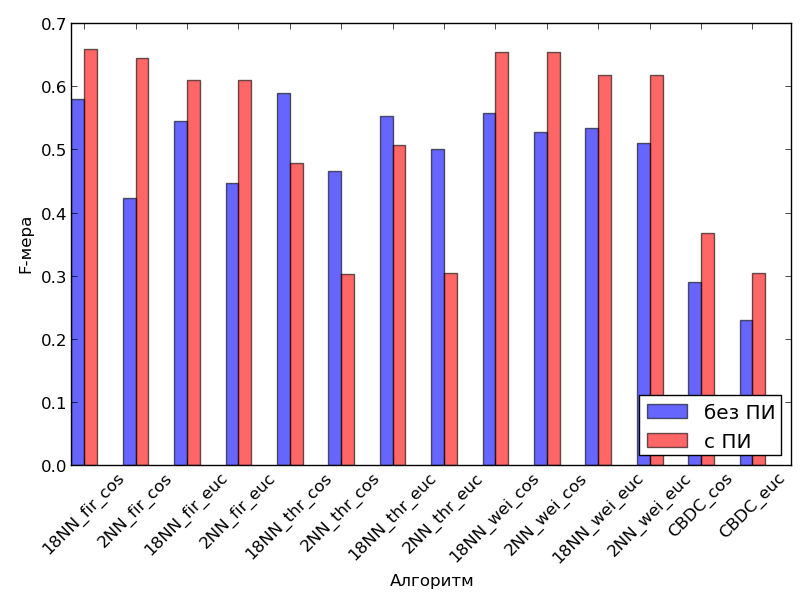
\includegraphics[width=170mm\textwidth]{persong.png}}
\caption{Гистограмма результатов запуска модификаций алгоритмов 2-NN, 18-NN и CBDC с применением перехода к исполнителю и без, 
persong-статистика, thresold = 0.250. ПИ \ld переход к исполнителю.}
\label{pic:persong}
\end{figure}

\begin{table}[ht]
\centering
\captionsetup{justification=centering}
\caption{Таблица с результатами запуска модификаций алгоритмов 2-NN, 18-NN и CBDC с применением перехода к исполнителю и без, perword-статистика, thresold = 0.250. ПИ \ld переход к исполнителю.}
\label{tab:annotation_perword}
\begin{tabular}{l c c ccc}
\hline\hline
 Алгоритм & Метрика & Исп.ПИ. & Precision & Recall & F-measure
\\ [0.5ex]
    \hline

    
    & & нет&$0.233$ & $0.306$ & $0.245$ \\[-1.5ex]
    \raisebox{1ex}{2NN(fir)} & \raisebox{1ex}{cos}
    & да &$0.309$ & $0.322$ & $0.315$ \\[2ex]

    & & нет&$0.236$ & $0.306$ & $0.245$ \\[-1.5ex]
    \raisebox{1ex}{18NN(fir)} & \raisebox{1ex}{cos}
    & да &$0.309$ & $0.322$ & $0.315$ \\[2ex]	

    & & нет&$0.205$ & $0.281$ & $0.236$ \\[-1.5ex]
    \raisebox{1ex}{2NN(fir)} & \raisebox{1ex}{euc}
    & да &$0.287$ & $0.308$ & $0.270$ \\[2ex]

    & & нет&$0.250$ & $0.281$ & $0.236$ \\[-1.5ex]
    \raisebox{1ex}{18NN(fir)} & \raisebox{1ex}{euc}
    & да &$0.287$ & $0.308$ & $0.270$ \\[2ex]

    & & нет&$0.223$ & $0.207$ & $0.202$ \\[-1.5ex]
    \raisebox{1ex}{2NN(wei)} & \raisebox{1ex}{cos}
    & да &$0.369$ & $0.416$ & $0.391$ \\[2ex]

    & & нет&$0.223$ & $0.207$ & $0.202$ \\[-1.5ex]
    \raisebox{1ex}{18NN(wei)} & \raisebox{1ex}{cos}
    & да &$0.369$ & $0.416$ & $0.391$ \\[2ex]

    & & нет&$0.222$ & $0.245$ & $0.221$ \\[-1.5ex]
    \raisebox{1ex}{2NN(wei)} & \raisebox{1ex}{euc}
    & да &$0.293$ & $0.286$ & $0.289$ \\[2ex]

    & & нет&$0.222$ & $0.245$ & $0.221$ \\[-1.5ex]
    \raisebox{1ex}{18NN(wei)} & \raisebox{1ex}{euc}
    & да &$0.293$ & $0.286$ & $0.289$ \\[2ex]

    & & нет&$0.307$ & $0.395$ & $0.340$ \\[-1.5ex]
    \raisebox{1ex}{CBDC} & \raisebox{1ex}{euc}
    & да &$\textbf{0.359}$ & $\textbf{0.392}$ & $\textbf{0.375}$ \\[2ex]

    & & нет&$0.329$ & $0.282$ & $0.302$ \\[-1.5ex]
    \raisebox{1ex}{CBDC} & \raisebox{1ex}{cos}
    & да &$0.327$ & $0.388$ & $0.351$ \\[2ex]
    
    & & нет&$0.259$ & $0.435$ & $0.325$ \\[-1.5ex]
    \raisebox{1ex}{2NN(thr)} & \raisebox{1ex}{cos}
    & да &$0.201$ & $0.823$ & $0.320$ \\[2ex]

    & & нет&$0.271$ & $0.435$ & $0.325$ \\[-1.5ex]
    \raisebox{1ex}{18NN(thr)} & \raisebox{1ex}{cos}
    & да &$0.223$ & $0.823$ & $0.320$ \\[2ex]

    & & нет&$0.302$ & $0.409$ & $0.347$ \\[-1.5ex]
    \raisebox{1ex}{2NN(thr)} & \raisebox{1ex}{euc}
    & да &$0.241$ & $0.859$ & $0.365$ \\[2ex]

    & & нет&$0.302$ & $0.409$ & $0.347$ \\[-1.5ex]
    \raisebox{1ex}{18NN(thr)} & \raisebox{1ex}{euc}
    & да &$0.243$ & $0.859$ & $0.365$ \\[2ex]
    \hline
\end{tabular}
\end{table}

\begin{figure}[h!]
\center{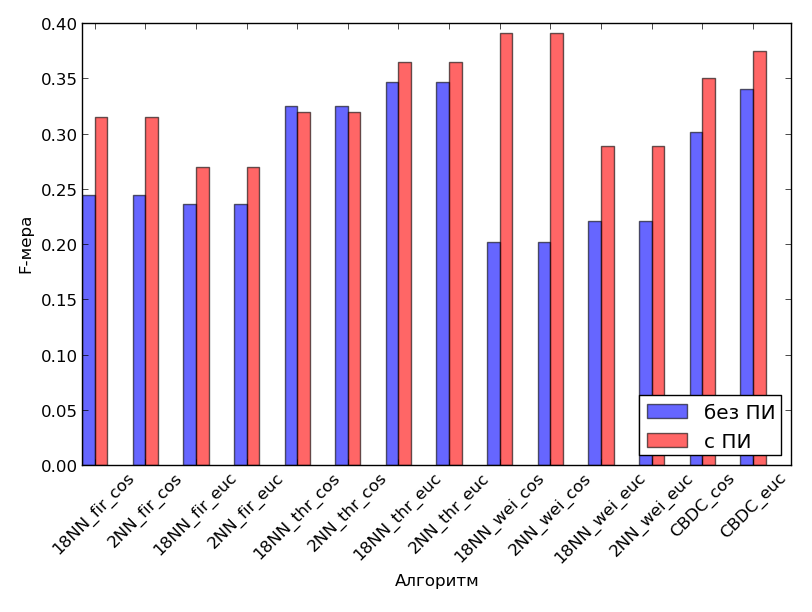
\includegraphics[width=170mm\textwidth]{perword.png}}
\caption{Гистограмма результатов запуска модификаций алгоритмов 2-NN, 18-NN и CBDC с применением перехода к исполнителю и без, perword-статистика, thresold = 0.250. ПИ \ld переход к исполнителю.}
\label{pic:perword}
\end{figure}

Как можно увидеть из таблицы \ref{tab:annotation_persong}, для первого (fir) и третьего (wei) способа фильтрации тегов алгоритмы с переходом к исполнителю показывают более высокие результаты.
В случае же второго способа фильтрации с введением порога переход к исполнителю дает сильный прирост лишь в полноте. Этот факт объясняется тем, что первый тег имеет такое значение в семантическом
веторе исполнителя, что следующий за ним в порядке убывания частоты появления среди всех треков уже не преодолевает выбранный порог. Если же увеличивать порог, то в алгоритме без перехода к исполнителю
во многих треках \emph{ни один} тег не преодолеет порог, и, как следствие, сравнивать два подхода будет уже нельзя.
Из таблицы \ref{tab:annotation_perword} видно, что при расчете статистики на тег, переход к исполнителю показывает более высокий результат и для F-меры для евлидовой метрики.

Исходя из полученных данных, можно сделать вывод, что переход к исполнителю для 2NN и для 18NN дает одинаковые результаты. Это объясняется тем, что самые основные теги, характеризующие исполнителя в целом, 
располагаются в самых первых соседях треков. Именно они и определяют первые теги в семантическом векторе исполнителя.

Стоит отметить, что лучший результат с использованием перехода к исполнителю при расчете на трек показал алгоритм 18NN(fir) с еквлидовой метрокий, а при расчете на тег \ld CBDC с косинусной метрикой.
В таблицах \ref{tab:annotation_persong} и \ref{tab:annotation_perword} соответствующие строки выделены жирным шрифтом.

\section{Эксперимент по поиску релевантных треков по тегу}

Цель данного эксперимента \ld проверить, как переход к исполнителю влияет на качество поиска релевантных треков по тегу.
Для этого мы упорядочиваем треки тестовой выборки по степени их ``принадлежности'' конкретному тегу. Чтобы оценить эту самую ``принадлежность'', в алгоритме k-NN используетя функция взвешивания.
Так как алгоритм CBDC для каждого тега возвращает расстояние $dist$ от его центра масс (см главу \ref{chapter1}) до конкретного трека, то мерой ``принадлежности'' в данном случае служит величина
$\max(dist) - dist$. Так, чем меньше расстояние, тем больше ``принадлежность''.

Для оценки качества тегирования и сравнения алгоритмов используются величины MeanAP (средняя по тегам площадь под precision-recall кривой) и MeanAROC (средняя по тегам площадь под ROC-кривой),
описанные в главе \ref{chapter1}. Подсчет производился кросс-валидацией, где $\frac{1}{10}$ часть обучающей выборки бралась для тестирования, а остальная \ld для тренировки.

В таблице \ref{tab:retrieval} приведены результаты работы алгоритмов с использованием перехода к исполнителю и без.
\begin{table}[ht]
\centering
\captionsetup{justification=centering}
\caption{Таблица с результатами применения алгоритмов 18-NN и CBDC для поиска треков по тегу с использованием перехода к исполнителю и без.}
\label{tab:retrieval}
\begin{tabular}{l c c ccc}
\hline\hline
 Алгоритм & Метрика & ПИ & MeanAP & MeanAROC
\\ [0.5ex]
    \hline

    
    & & нет&$0.431$ & $0.596$ \\[-1.5ex]
    \raisebox{1ex}{18NN} & \raisebox{1ex}{cos}
    & да &$\textbf{0.637}$ & $\textbf{0.651}$ \\[2ex]

    & & нет&$0.376$ & $0.617$ \\[-1.5ex]
    \raisebox{1ex}{18NN} & \raisebox{1ex}{euc}
    & да &$0.560$ & $0.646$ \\[2ex]

    & & нет&$0.397$ & $0.584$ \\[-1.5ex]
    \raisebox{1ex}{CBDC} & \raisebox{1ex}{cos}
    & да &$0.593$ & $0.645$ \\[2ex]

    & & нет&$0.265$ & $0.502$ \\[-1.5ex]
    \raisebox{1ex}{CBDC} & \raisebox{1ex}{euc}
    & да &$0.334$ & $0.513$ \\[2ex]

    \hline
\end{tabular}
\end{table}

Как видно из таблицы \ref{tab:retrieval}, во всех случаях переход к исполнителю дает более хорошие результаты.

Стоит отметить, что предложенный Mohamed Sordo метод CBDC в евлидовой метрике не показывает столь хороших результатов, как на CAL500.
Действительно, значение MeanAROC близко к $\frac{1}{2}$, что эквивалентно алгоритму со случайным выбором тегов.

Лучший результат показал алгоритм 18NN, соответствующие значения выделены жирным шрифтом.

\section{Выводы}

В данной главе была описана размеченная выборка с русской музыкой и описаны эксперименты. Проводилось два эксперимента \ld по сопоставлению тегов треку и по поиску релевантных треков по треку.
Было проведено сравнение методов автоматического тегирование с использованием перехода к исполнителю и без. Практически во всех случаях предложенный в данной работе метод показал более хорошие
результаты.
\chapter{Апробация} 
\label{approbation}

В данной главе будет описан подход к решению задачи в рекомендациях музыки социальной сети ``Одноклассники'', основанный на переходе
от трека к исполнителю, а также будут приведены результаты, показывающие улучшение рекомендаций после апробации данного подхода.

\section{Музыкальный сервис социальной сети “Одноклассники”}

Музыкальный сервис социальной сети ``Одноклассники'' доступен каждому зарегистрированному пользователю. Среди многочисленных возможностей, 
которые осуществляет сервис, имеются также рекомендации песен и исполнителей, формирование индивидуальных радиостанций. Устроены они на 
основе \emph{коллаборативной фильтрации}~\cite{bugaychenko}. То есть для определения вкусов пользователей и рекомендации им подходящей музыки анализируется 
их активность в музыкальном сервисе: что слушал человек, как долго, в каком порядке, как много раз, что из прослушанного было добавлено 
в собственные списки, какие треки слушались подряд и так далее. Затем на основе этой информации определяются \emph{похожие} треки и исполнители,
которые и попадают в списки рекомендаций. Например, если зайти на страницу с музыкой какого-либо исполнителя, то вниманию пользователя будут 
предложены не только его песни, но 16 похожих на него исполнителей.

\section{Проблема определения похожих исполнителей}

На портале регулярно происходит обновление списка пар похожих исполнителей, в процессе которого пересчитываются коэффициенты ``похожести''.
Как уже отмечалось, на эти коэффициенты влияет пользовательская активность. Таким образом поддерживается актуальность рекомендаций.
Так как люди могут слушают музыку из разных направлений, обладать разносторонними вкусами, то в списки рекомендаций могут попадать совершенно
непохожие исполнители. Например, похожими считаются некоторые российские исполнители поп-музыки и шансона. 
Более наглядные примеры, когда на странице исполнителя современного джаза рекомендуется русская поп-музыка, или же 
на странице симфо-метал исполнителя в списках похожих показывается хип-хоп исполнители.

Объяснить подобные ``промахи'' можно следующим образом: большинство людей вне зависимости от своих вкуснов все же слушают современную популярную
музыку, мешая ее в плейлистах с более узкими жанрами \ld рэп, метал, классика. Поэтому если большое количество любящих минимал-техно пользователей 
прослушают новую песню российской поп-музыки, то она покажется рекомендательной системе похожей на ту музыку, которую обычно слушают эти пользователи. 

Чтобы указать на еще одну причину подобного смешения рекомендаций, рассмотрим в качестве примера рэпкор-группу Crazy Town, которая появляется в 
рекомендациях у некоторых поп-исполнителей, несмотря на направление музыки данной группы \ld ню-метал, рэп-рок, альтернативный рок. Дело в том,
что у данной группы есть песни-хиты, которые популярны в широкой публике, а не только среди любителей перечисленных выше жанров. Одной из таких песен
является ``Butterfly'', которую слушают вместе с остальной популярной музыкой. Благодаря этому данная группа считается похожей на исполнителей
совершенно других направлений.

Таким образом возникает следующая задача: отфильтровать списки рекомендаций, полученные коллаборативной фильтрацией, убрав из них пары заведомо 
непохожих исполнителей.

\section{Описание предлагаемого подхода}

Поставим задачу более формально. Имеется пара исполнителей, которые коллаборативная рекомендательная система посчитала похожими. 
Необходимо определить, являются ли эти исполнители \emph{непохожими}, либо пропустить эту пару. 

Предлагаемый для решения поставленной задачи подход основан на переходе от тегов трека к тегам исполнителя с некоторыми модификациями, 
связанными с особенностями поставленной задачи. 

Сначала все теги разделяются на \emph{кластеры} \ld множества тегов, которые
часто ассоциируются с одним и тем же треком \emph{одновременно}. Этот процесс можно сравнить с выделением синонимичных тегов, о которых
шла речь в \cite{msordo_thesis}. Для этого предлагается построить неориентированный взвешенный граф, вершинами которого являются теги, а весом ребра между
тегами $w_1$ и $w_2$ является величина
$$ \max \left ( \frac{|w_1 \cap w_2|}{|w_1|}, \frac{|w_1 \cap w_2|}{|w_2|} \right ) $$,
где $|w_1|, |w_2|$ \ld количество треков, помеченных тегами $w_1, w_2$ соответственно, $|w_1 \cap w_2|$ \ld количество треков, 
помеченных обоими тегами сразу. Затем в графе отбрасываются ребра, вес которых ниже определенного порога, получаемого эмпирически с 
использованием экспертной оценки объединенных тегов. Например, в нашем случае требовалось, чтобы теги ``хип-хоп'' и ``рэп''
были в одном кластере, а ``метал'' и ``классика'' \ld в разных. Пусть теперь имеется треки $t_1$ и $t_2$, и с ними ассоциированы множества тегов
$W_1, W_2$ соответственно. Пусть также $C_1, C_2$ \ld множества кластеров, которым принадлежат теги из $W_1, W_2$ соответственно. 
Так как теги разных кластеров ассоциируются с одной и той же песней достаточно редко, то логично предположить, что если $C_1 \cap C_2 = \varnothing$, 
то данные треки скорее всего не похожи. Действительно, если трактовать данное разбиение на кластеры как выделение схожих 
музыкальных направлений, то в таком случае эти треки будут принадлежать разным направлениям.

В итоге, чтобы отфильтровать непохожих исполнителей, необходимо:
\begin{itemize}
 \item протегировать треки исполнителей;
 \item выполнить переход к каждому из исполнителей;
 \item определить кластеры, к которым относятся теги исполнителей;
 \item если множества кластеров не пересекаются, то считать исполнителей непохожими.
\end{itemize}

\section{Результаты}

Проверке на похожесть подверглось около 17 миллионов пар исполнителей. На каждого исполнителя бралось от 6 до 10 треков. Тегирование производилось 
алгоритмом $k$-NN с косинусной метрикой при $k = 18$. Словарь состоял из 27 жанровых тегов, которые разбились на 15 кластеров.
Для оценки качества предложенной фильтрации было вручную выбрано 200 пар исполнителей, среди которых 100
были похожими, а другие 100 \ld нет. В результате фильтрации из 100 похожих исполнителей осталось 93, а из 100 непохожих \ld 8.
Применение данной дополнительной фильтрации повлияло не только на рекомендации, но и на формирование пользовательских радиостанций.
Например, в радиостанции ``Индастриал-метал'' перестала попадаться поп-музыка.

\section{Выводы}

В данной главе была сформулирована проблема фильтрации непохожих исполнителей в социальной сети ``Одноклассники''. Также был сформулирован подход к ее решению
на основе перехода к исполнителю и выделения кластеров с тегами. Данный метод был внедрен в существующую фильтрацию и показал хорошие результаты.
% \startconclusionpage

В данной работе было проведено исследование существующих алгоритмов ближайших соседей, 
а также был предложен новый подход к автоматическому тегированию \ld переход к от трека к исполнителю.
При данном переходе для тегирования конкретного трека используется не только информация о нем самом,
но и теги других треков того же исполнителя. Таким образом стало возможно исправлять отдельные плохо 
протегированные треки, увеличивая качество тегирования в целом.
Для проверки данного подхода были проведены эксперименты по тегированию русской музыки с использованием
экспертно составленной выборки. Данные эксперименты показали, что использование предложенного метода 
привело к заметному увеличению точности тегирования как в задаче сопоставления тегов треку, так и в задаче поиска треков
по тегу, практически во всех исследованных вариациях алгоритмов $k$-NN и CBDC.
Переход от тегов трека к тегам исполнителя был успешно применен для фильтрации похожих исполнителей в 
рекомендациях музыкального сервиса социальной сети ``Одноклассники''.

Таким образом, данная работа полностью удовлетворяет поставленным требованиям.

В качестве дальнейшей работы предлагается исследование перехода к исполнителю применительно к другим
алгоритмам тегирования, основанным, например, на SVM, GMM, нейронных сетях и так далее. Также возможен
поиск способа учитывать при переходе к исполнителю и индивидуальные особенности треков.



% \printbibliography

\end{document}
